%%%%%%%%%%%%%%%%%%%%%%%%%
%                                                 %
%                 Experiment M-8                  %
%         Experiment Title  Rotational Motion     %
%                                                 %
%%%%%%%%%%%%%%%%%%%%%%%%%

%\labChapter{M}{[1171L] - Rotational Motion}
\labChapter{M}{[1171L - CALC-BASED course] --- Rotational Dynamics with Moment of Inertia \& Angular Momentum}
\label{lab:M7_1171L}

% Introduction
%\section{Introduction}
% Background
\section{Background}

The motion of an object can be divided into two, completely independent parts: the linear (translational) motion of the center of mass and the rotational motion of the object around an axis through the center of mass. The linear motion is explained by Newton's 2nd Law of motion: a net force $F_{net}$ acting on an object of mass $m$ will cause the object to experience a linear acceleration $a$ given by
\[
F_{net} = m a.
\]
Rotational motion can be described in a very similar manner, but the quantities involved need to be changed to rotational quantities. These quantities are described and explained in detail in the following paragraphs.



% Moment of Inertia
\subsection{Moment of Inertia}

In rotational motion the moment of inertia (usually denoted by $I$) takes the role of mass. An object with a large value of $I$ will be reluctant to change its rotational motion. Just as mass this quantity is a scalar, meaning that it has no direction. The moment of inertia of a system of objects can be determined easily by adding the moment of inertia of each of the different components making up the entire system. The moment of inertia depends not only on the mass of the object but also on how the mass is distributed with respect to the axis of rotation. The further the mass is away from the axis of rotation, the higher the moment of inertia will be. For a point mass (an object that can be considered small with respect to its distance from the axis of rotation) the moment of inertia is defined as
\begin{equation}
  \label{eq:M08pointMass}
  I = m\, R^{2}
\end{equation}
where $m$ is the mass of the object and $R$ is the distance of the object from the axis of rotation.
The calculation of the moment of inertia for more complex objects is a rather straightforward process, but can be very tedious. In most cases simple expressions can be found to calculate the value of $I$. The list below gives the moment of inertia for a few objects used in this lab:

\begin{itemize}
\item[$\triangleright$] A \textbf{solid disk} of mass $M_{D}$ and radius $R_{D}$ rotating about an axis through its center: 
  \begin{equation}
    \label{eq:M08Idisk}
    I= \frac{1}{2} M_{D} \, R_{D}^{2}
  \end{equation}
\item[$\triangleright$] A \textbf{thin-walled ring} of mass $M_{R}$ and radius $R_{R}$ rotating about an axis through its center: 
  \begin{equation}
    \label{eq:M08Ithinring}
    I= M_{R} \, R_{R}^{2}
  \end{equation}
\item[$\triangleright$] A \textbf{thick ring} mass $M_{R}$ and inner radius $R_{i}$ and outer radius $R_{o}$ rotating about an axis through its center:
  \begin{equation}
    \label{eq:M08Ithickring}
    I=\frac{1}{2} M_{R} \, \left(R_{i}^2 + R_{o}^2\right)
  \end{equation}
\end{itemize}

% Torque
\subsection{Torque}

A force by itself is not enough to determine whether an object will start to rotate (just think about how a force that is applied to the hinges of a door will not rotate the door). Instead we define a new quantity, called torque $\tau$, which combines the force and the distance from the axis of rotation (also called the lever arm). This quantity is a vector quantity, meaning that it does have a direction
\begin{equation}
  \vec{\tau} = \vec{F}_{\perp} \times \vec{d}.
\end{equation}
Here $\vec{d}$ denotes the lever arm (directed outward from the center) and $\vec{F}_{\perp}$ is the component of the force perpendicular to the lever arm.

% Newton's 2nd Law for Rotational Motion
\subsection{Newton's 2nd Law for Rotational Motion}

With the above definitions we can now formulate a rotational version of Newton's 2nd Law. An object with moment of inertia $I$ will experience an angular acceleration $\vec{\alpha}$, if a net torque $\vec{\tau}_{\mbox{net}}$ acts on it
\begin{equation}
  \vec{\tau}_{\mbox{net}} = I \vec{\alpha}.
\end{equation}


\pagebreak 
% Calculating the moment of inertia
\subsection{Calculating the Moment of Inertia}

One can use Newton's 2nd Law for Rotational Motion to calculate the moment of inertia of an object from the angular acceleration $\alpha$ and the net torque acting on the object.
\[
I = \frac{\left|\vec{\tau}_{\mbox{net}}\right|}{\left|\vec{\alpha}\right|}
\]



The simplified sketch in Fig.~\ref{M08Fig01} shows the setup used in this lab.
The net torque acting on the pulley can be written as
\[
|\vec{\tau}_{\mbox{net}}| = T \, R_{P}
\]
where $T$ is the tension in the string and $R_{P}$ is the radius of the 3-step pulley. Since the tension is not known it has to be determined from the linear acceleration a of the hanging mass, using the net force acting on the mass $m$ (see force diagram in the sketch):
\[
F_{\mbox{net}} = m g - T = m a.
\]
In addition the linear acceleration $a$ is related to the angular acceleration $\alpha$ by
\[
a = \alpha R_{P}.
\]

Using this set of equations one can now solve for the moment of inertia, $I$,
\begin{equation}
  \label{eq:M08Eq03}
  I = \frac{m \left(g  R_{P} - \alpha R_{P}^2\right)}{\alpha}.
\end{equation}


\begin{figure}
  \begin{center}[h]
    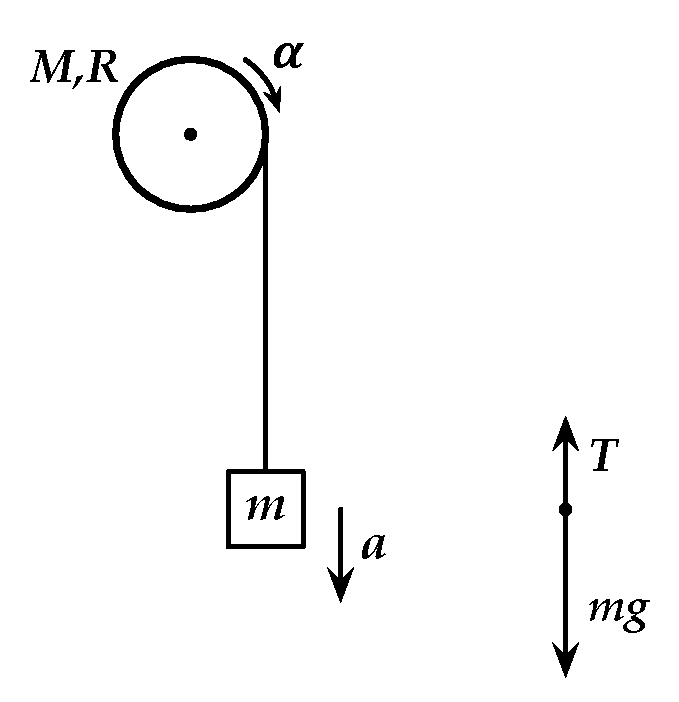
\includegraphics[width=2.2in]{Experiment09Figures/Figure01.pdf}
  \end{center}
  \caption{Left: Sketch of a pulley of mass $M$ and radius $R$ being accelerated by a hanging mass $m$. Note that the pulley in the lab is actually horizontal, but is drawn vertically here for simplicity. Right: Force diagram for the hanging mass $m$.}
  \label{M08Fig01}  % the \label command comes AFTER the caption
\end{figure}




% Angular Momentum
\subsection{Angular Momentum}

A similar derivation as above can be used to define the quantity of angular momentum $\vec{L}$ from the definition of linear momentum ($\vec{p} = m \vec{v}$)
\[
|L| = I \omega
\]
Angular momentum is conserved (meaning it will not change its value) if there is no external torque acting on a system
\[
\vec{L}_i = {L}_f.
\]
This can be used to determine the angular velocity of a system if the moment of inertia changes
\begin{equation}
  I_i \omega_i = I_f \omega_f.
\end{equation}


\textbf{THE PARALLEL AXIS THEOREM} is used to calculate the moment of inertia of an object of mass $M$ rotating about a rotation axis that does not pass through the center of mass (e.g. the ring on top of the apparatus is off center). The moment of inertia for the axis ${I_{axis}}$  is
\begin{equation}
\label{M7RotationalMotion_OffAxis}
    {I_{axis}} = {I_{ring}} + M d_{cm}^2
\end{equation}
where ${I_{cm}}$ is the moment of inertia about an axis through the center of mass parallel to the rotation axis. The distance between the parallel axes is ${d_{cm}}$. In the Conservation of Angular Momentum experiment you drop the ring on the rotating apparatus.  Although you try to drop the ring centered on the axis of rotation, it often lands off center. You will run a case where you try to center it, and then another case where you purposefully drop it off center.


\section{Experimental Procedure}

The experiment makes use of a sensor, which is able to detect and measure angular displacement, angular velocity, and angular acceleration. This Rotary Motion Sensor (RMS), with a \textbf{stated uncertainty of 0.09\degree}, is attached to a vertical rod and has a 3-step pulley affixed to its axle (see Fig.~\ref{M08Fig02}). Objects with different moment of inertia can be mounted onto the 3-step pulley and their rotational motion be measured. A second pulley (called a Super Pulley) is attached to the RMS to allow a string to spool off the 3-step pulley as shown in Figures~\ref{M08Fig02} and ~\ref{M08Fig03}. A weight hanger of known mass $m$ is attached to the free end of the string and provides an accelerating torque to the 3-step pulley and therefore to the object mounted on it.

In this experiment you will measure the angular acceleration from a graph of angular velocity vs. time using data recorded with the RMS. The data will be collected in \textbf{Capstone}, which also provides analysis tools. %See page~\ref{sec:SettingUpHardware} for guidance. 
The moment of inertia of a ring and of two point masses will be determined from the angular acceleration. Finally, you will verify the validity of angular momentum conservation in an inelastic collision.

\begin{figure}
  \begin{center}
    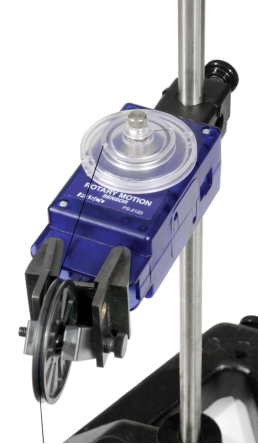
\includegraphics[width=2.2in]{Experiment09Figures/Figure02.pdf}
  \end{center}
  \caption{Rotary Motion Sensor (RMS) with 3-step pulley (transparent) and Super Pulley (black).}
  \label{M08Fig02}
\end{figure}

\begin{figure}
  \begin{center}
    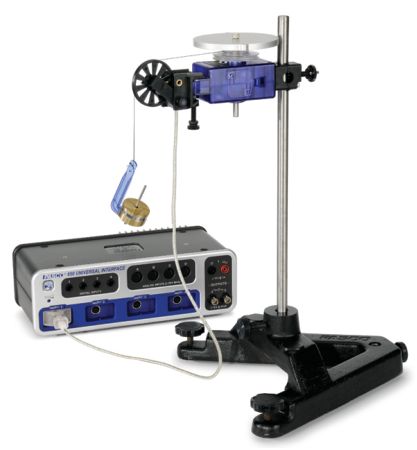
\includegraphics[width=2.4in]{Experiment09Figures/Figure03a.pdf}
    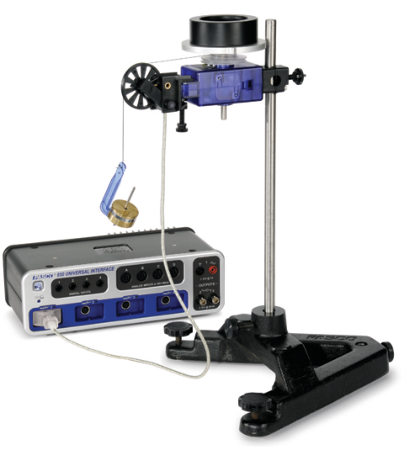
\includegraphics[width=2.4in]{Experiment09Figures/Figure03b.pdf}
  \end{center}
  \caption{Experimental setup of the RMS apparatus with disk alone (left) and with disk and ring mounted (right). The setup varies slightly from the one used in the lab.}
  \label{M08Fig03}
\end{figure}

% Moment of Inertia of the Ring
\subsection{Moment of Inertia of the Ring}

In Part~1 of the experiment you will measure the moment of inertia of the ring and of the apparatus by measuring angular acceleration with a known torque.
\begin{itemize}
\item[$\triangleright$] Create a Part~1 Data Table for your measurements and calculations of the moment of inertia of the ring.
\item[$\triangleright$] Determine the mass of the ring and note the result as $M_{\mbox{ring}}$ in your Part~1 Data Table.
\item[$\triangleright$] Measure the inner and outer radii of the ring, using the calipers. See the instructions at Fig.~\ref{VernierFig02} for using the Vernier caliper. Note the result as $R_{i}$ and $R_{o}$ in your Part~1 Data Table.
\item[$\triangleright$] Calculate the expected moment of inertia of the ring, using Eqn.~\ref{eq:M08Ithickring} given in the Background. Note your result as $I_{\mbox{calc}}$ in your Part~1 Data Table.
\item[$\triangleright$] Place the ring onto the disk, which should already be mounted on the Rotary Motion Sensor (RMS). The two pins of the ring should fit into the two holes on the disk.
\item[$\triangleright$] Note the mass of the hanger as $m$ in your Data Table.
\item[$\triangleright$] Using the calipers measure the radius $R_{P}$ of the smaller pulley of the RMS and note your result in your Part~1 Data Table. See the instructions at Fig.~\ref{VernierFig02} for using the Vernier caliper.
\item[$\triangleright$] Wind the string with the attached mass hanger onto the smaller pulley of the RMS. You need to make sure that the string runs over the Super Pulley, is wound nicely onto the smaller pulley of the RMS, and is leaving the pulley of the RMS tangentially before it runs straight over the Super Pulley.
\item[$\triangleright$] Measure the angular acceleration $\alpha_{\mbox{total}}$ of the ring plus the apparatus (the disk and the RMS).
  \begin{enumerate}
  \item Make sure that in \textbf{Capstone} you have a graph of angular velocity ($y$-axis) vs. time ($x$-axis) open.
  \item Before releasing the mass hanger press the \textbf{Record} button on \textbf{Capstone}.
  \item Release the mass hanger and note that the recorded graph is a straight line.
  \item Press the \textbf{Record} button again right before the string is completely unwound from the pulley to stop recording any more data points.
  \item Using the \textbf{Fit} option in \textbf{Capstone}, fit a straight line (linear fit) to the data, in the region where the system is accelerating (highlight the data region in the graph you want to fit).
  \item The slope of this graph is the angular acceleration $\alpha_{\mbox{total}}$.
  \item Note your result in your Data Table.
  \end{enumerate}
\item[$\triangleright$] Calculate the moment of inertia of the apparatus plus the ring, using Eqn.~\ref{eq:M08Eq03} given in the Introduction. Note your result as $I_{\mbox{total}}$ in your Part~1 Data Table.
\item[$\triangleright$] Remove the ring from the apparatus and repeat the above steps to determine the moment of inertia of the apparatus without the ring. Note the results as $\alpha_{\mbox{app}}$ and $I_{\mbox{app}}$ in your Data Table.
\item[$\triangleright$] To determine the moment of inertia of the ring subtract $I_{\mbox{app}}$ from $I_{\mbox{total}}$. Note your result as $I_{\mbox{exp}}$ in your Data Table.
\item[$\triangleright$] Repeat the above measurements three times.
\item[$\triangleright$] Calculate averages and standard deviations $\sigma(I)$ for the moments of inertia.% (See Eqn.~\ref{eq:errorSigmaX}).
\item[$\triangleright$] Compare the difference between your calculated value and the experimental value with its uncertainty.
\end{itemize}

% Moment of Inertia of two point masses
\subsection{Moment of Inertia of Two Point Masses}
In Part~2 of the experiment, you will measure the moment of inertia of two point masses on a rod. 
\begin{itemize}
\item[$\triangleright$] Create a Part~2 Data Table for your measurements and calculations of the moment of inertia of the point masses.
\item[$\triangleright$] Please call the lab instructor for this: Mount the rod onto the pulley of the RMS.
\item[$\triangleright$] Determine the masses of the two brass weights (with screws) and note the result as $M_1$ and $M_2$ in your Data Table.
\item[$\triangleright$] Mount the masses into the end of the rod and fasten them with the screws. Measure the distance of the center of the masses from the center of the rod. Note the results as $R_1$ and $R_2$ in your Data Table.
\item[$\triangleright$] Calculate the expected moment of inertia of the two points masses, using Eqn.~\ref{eq:M08pointMass} given in the Introduction. Note your result as $I_{\mbox{calc}}$ in your Data Table.
\item[$\triangleright$] Note the mass of the hanger as $m$ in your Data Table.
\item[$\triangleright$] Note the radius $R_{P}$ of the smaller pulley of the RMS in your Data Table (use the result from Part~1 above).
\item[$\triangleright$] Wind the string with the attached mass hanger onto the smaller pulley of the RMS. You need to make sure that the string runs over the Super Pulley, is wound nicely onto the smaller pulley of the RMS, and is leaving the pulley of the RMS tangentially before it runs straight over the Super Pulley.
\item[$\triangleright$] Measure the angular acceleration $\alpha_{\mbox{total}}$ of the two masses plus the apparatus (the rod and the RMS):
  \begin{enumerate}
  \item Make sure that in \textbf{Capstone} you have a graph of angular velocity ($y$-axis) vs. time ($x-axis$) open.
  \item Before releasing the mass hanger press the \textbf{Record} button on \textbf{Capstone}.
  \item Release the mass hanger and observe the recorded data points/graph.
  \item Press the \textbf{Record} button again right before the string is completely unwound from the pulley to stop recording any more data points.
  \item Discuss (among yourselves and with your instructor) the resulting graph before continuing.
  \item Using the \textbf{Fit} option in \textbf{Capstone}, fit a straight line (linear fit) to the data, in the region where the system is accelerating (highlight the data region in the graph you want to fit).
  \item The slope of this graph is the angular acceleration $\alpha_{\mbox{total}}$.
  \item Note your result in your Data Table.
  \end{enumerate}
\item[$\triangleright$] Calculate the moment of inertia of the apparatus plus the two point masses, using Eqn.~\ref{eq:M08Eq03} given in the Introduction. Note your result as $I_{\mbox{total}}$ in your Data Table.
\item[$\triangleright$] Remove the two point masses from the apparatus and repeat the above steps to determine the moment of inertia of the apparatus without the two masses. Note the result as $I_{\mbox{app}}$ in your Data Table. Please note that you need to again discuss the collected data points/graph with your lab instructor.
\item[$\triangleright$] To determine the moment of inertia of the two point masses subtract $I_{\mbox{app}}$ from $I_{\mbox{total}}$. Note your result as $I_{\mbox{exp}}$ in your Data Table.
\item[$\triangleright$] Repeat the above measurements three times.
\item[$\triangleright$] Calculate averages and standard deviations $\sigma(I)$ for the moments of inertia.% (See Eqn.~\ref{eq:errorSigmaX}).
\item[$\triangleright$] Compare the difference between your calculated value and the experimental value with its uncertainty.
\end{itemize}


\pagebreak

% Conservation of Angular Momentum
\subsection{Conservation of Angular Momentum}
In Part~3 of the experiment you will observe the conservation of angular momentum in an inelastic collision. 
\begin{itemize}
\item[$\triangleright$] Create a Part~3 Data Table for your measurements and calculations of the conservation of angular momentum.
\item[$\triangleright$] Please call the lab instructor for this: Mount the disk onto the pulley of the RMS.
\item[$\triangleright$] Copy the result of the moment of inertia of the ring ($I_{\mbox{ring}}$) from the Part~1 Data Table to your Part~3 Data Table.
\item[$\triangleright$] Copy the result of the moment of inertia of the apparatus, which includes the mounted disk ($I_{\mbox{app}}$) from the Part~1 Data Table your Part~3 Data Table.
\item[$\triangleright$] Hold the ring with the pins facing up just above the center of the disk.
\item[$\triangleright$] Practice the drop a few times before continuing:
  \begin{enumerate}
  \item Give the disk a spin with your hand.
  \item Hold the ring a few millimeters above the spinning disk centered on the axis of the disk. 
  \item Drop the ring onto the spinning disk, so that the ring is centered on the disk.
  \end{enumerate}
\item[$\triangleright$] Measure the angular speeds $\omega_{i}$ and $\omega_{f}$ (before and after dropping the ring onto the disk):
  \begin{enumerate}
  \item Make sure that in \textbf{Capstone} you have two graphs of angular position ($y$-axis) vs. time ($x$-axis) and of angular velocity ($yu$-axis) vs. time ($x$-axis) open.
  \item Make sure that in \textbf{Capstone} you have a data table of the angular velocity open.
  \item Give the disk a spin with your hand and press the \textbf{Record} button on \textbf{Capstone}, while still holding the ring above the (now spinning) disk.
  \item Record about 25 data points (about 2--3 seconds), then let the disk drop onto the disk.
  \item Press the \textbf{Record} button again after collecting about 25 more points (again about 2--3 seconds).
  \item Using the \textbf{Fit} option in \textbf{Capstone}, fit a straight line (linear fit) to the angular position vs. time graph, in the two data regions (highlight the data region in the graph you want to fit).
  \item The two slopes are the angular velocities $\omega_i$ and $\omega_f$.
  \item Discuss among yourselves and with your instructor why this will not be a good determination of the speeds $\omega_i$ and $\omega_f$.
  \item Among yourselves and with your instructor discuss a better way to determine the speeds (Hint: Think about the exact instant at which you need to determine the speeds). Explain why your new method is better than the one mentioned above.
  \item Note the final results for the speeds $\omega_i$ and $\omega_f$ in your Part~3 Data Table.
  \end{enumerate}
\item[$\triangleright$] Calculate the angular momentum of the disk-ring system before the ring is dropped onto the disk. Note your result as $L_i$ in your Data Table.
\item[$\triangleright$] Calculate the angular momentum of the disk-ring system after the ring is dropped onto the disk. Note your result as $L_f$ in your Data Table.
\item[$\triangleright$] Compare the difference between your calculated value and the experimental value with its uncertainty.

\item Parallel Axis Theorem test:
\begin{itemize}
    \item Run an additional test of the angular momentum part where you drop the ring to purposefully be off center.
    \item Measure the off-center distance ${d_{cm}}$ when the ring is all the way against the main axis of rotation of the metal plate (i.e. inner edge of the ring against the screw).
    \item Calculate the updated moment of inertia of the ring using the parallel axis theorem, Eqn.~\ref{M7RotationalMotion_OffAxis}.
    \item Spin the disk as fast as possible and drop the ring off center to the point where it ends up against the screw, akin to what you just measured for ${d_{cm}}$.
    \item Record both the initial and final angular velocities.
    \item Calculate both the initial and final angular momentum.
\end{itemize}

\end{itemize}


\section{Data Analysis}
The first experiment determines the moment of inertia of the ring by measuring its angular acceleration.
\begin{itemize}
\item[$\triangleright$] Create a table to find $I_{\mbox{calc}}$ including
  \begin{itemize}
  \item the ring mass $M_{\mbox{ring}}$,
  \item the inner and outer radii of the ring,
  \item the calculated moment of inertia $I_{\mbox{calc}}$.
  \end{itemize}
\item[$\triangleright$] Create a table to find $I_{\mbox{exp}}$ including
  \begin{itemize}
  \item the hanging mass $m$,
  \item the radius of the pulley $R_P$,
  \item the angular acceleration and calculated moment of inertia with the ring and apparatus,
  \item the angular acceleration and calculated moment of inertia of the apparatus,
  \item the experimental moment of inertia of the ring $I_{\mbox{exp}}$.
  \end{itemize}
\end{itemize}

The second experiment determines the moment of inertia of a rod with two masses by measuring its angular acceleration.
\begin{itemize}
\item[$\triangleright$] Create a table to find $I_{\mbox{calc}}$ including
  \begin{itemize}
  \item the masses $M_1$ and $M_2$,
  \item the radii $R_1$ and $R_2$,
  \item the calculated moment of inertia of the masses $I_{\mbox{calc}}$.
  \end{itemize}
\item[$\triangleright$] Create a table to find $I_{\mbox{exp}}$ including:
  \begin{itemize}
  \item the hanging mass $m$,
  \item the radius of the pulley $R_P$,
  \item the angular acceleration and calculated moment of inertia of the apparatus (rod) and masses,
  \item the angular acceleration and calculated moment of inertia of the apparatus,
  \item the experimental moment of inertia of the masses $I_{\mbox{exp}}$.
  \end{itemize}
\end{itemize}

The third experiment in this lab shows conservation of angular momentum by illustrating the change in angular velocity with an increase in moment of inertia.
\begin{itemize}
\item[$\triangleright$] Create a table of common data $I_{\mbox{ring}}$ and $I_{\mbox{app}}$.
\item[$\triangleright$] Create a table with a row for each trial including
  \begin{itemize}
  \item the initial angular velocity, $\omega_i$,
  \item the final angular velocity, $\omega_f$,
  \item the initial angular momentum, $L_i$,
  \item the final angular momentum, $L_f$,
  \item the change in angular momentum, $\Delta L$.
  \end{itemize}
\end{itemize}


\pagebreak

\section{Post-Lab Submission --- Interpretation of Results}

\begin{itemize}
    \item Make sure to submit your finalized data table (Excel sheet)
    \item Part 1: How do the values of both the \textbf{ring's} and \textbf{two-point masses'} measured I compare to the “predicted (from geometry)” value? Treating your standard deviations as your uncertainty, do your results span the difference between experimental and theoretical, thereby agreeing?
    \item Part 1 (empty rod): In the part of the experiment measuring the moment of inertia of the rod apparatus without the weights, notice that the rod turns quite fast and that the angular acceleration decreases as the speed increases (see plot in \textbf{Capstone}). Why does this happen?
    \item Part 2: Is angular momentum $L$ conserved? What might cause any discrepancies in the conservation of angular momentum?
    \item Part 2: What is the effect of dropping the ring off-center? Is L conserved when considering the off-axis portion?
    \item What are your measurement uncertainties for each experiment?
    \item What are possible systematic uncertainties for each experiment?
\end{itemize}





